\documentclass[12pt,fleqn]{article}
\setlength{\parindent}{0pt}
\usepackage{graphicx}
\usepackage{cancel}
\usepackage{listings}
\usepackage[latin5]{inputenc}
\usepackage{color}
\setlength{\parskip}{8pt}
\setlength{\parsep}{0pt}
\setlength{\headsep}{0pt}
\setlength{\topskip}{0pt}
\setlength{\topmargin}{0pt}
\setlength{\topsep}{0pt}
\setlength{\partopsep}{0pt}
\setlength{\mathindent}{0cm}
\usepackage{latexsym}
\usepackage{amsfonts}
\usepackage{showkeys}
\renewcommand*\showkeyslabelformat[1]{(#1)}

\begin{document}
Ders 1

Dersin kullanacagi ana kitap L. C. Evans'in Kismi Turevsel Denklemler
(partial differential equations -PDE-) kitabi olacak. Bir sonraki ders icin
okuma odevi soyle:

1. Sf. 1-13'teki ozet

2. Alt bolum 2.1 sf. 17-19

3. Bolum 3 sf. 91-115 arasini tamamen. 

PDE'leri incelerken cogunlukla onlarin temsil ettigi fiziksel fenomenleri
de inceleyecegiz. Mesela transportasyon (transport) denklemleri, ki

\[ \partial_t u + \vec{b} \cdot \vec{\nabla} u = 0 \]

Ustteki ifadede gradyan operatoru var, bu bilindigi gibi

\[ \vec{\nabla} = \bigg( 
\frac{\partial }{\partial x_1},.., 
\frac{\partial }{\partial x_n},
\bigg)
\]

$\vec{b}$ icinde sabitler olan bir vektor olabilir

\[ \vec{b} = (b_1,...,b_n)
 \]

Bu denklem 1. derece PDE'lerin ozel bir durumudur bu arada. 1. derece
PDE'ler 

\[ F(x, u(x), Du(x)) = 0 \]

seklindedir. $D$ notasyonu Evans'in gradyan icin kullandigi notasyon,
alissak iyi olur. Yani

\[ Du = \nabla u \]

Ustteki gibi denklemlere bakacagiz, cozumlerini gorecegiz. Mesela ustteki
denklem direk ODE yaklasimi ile cozulebiliyor. Bu hakikaten ilginc bir sey,
yani ustteki gibi genis bir PDE kategorisi, $n$ tane degisken icerebilen
turden denklemler ODE'lere indirgenerek cozulebiliyor. Bu yonteme
``karakteristikler metotu (method of characteristics)'' ismi veriliyor.

Bu arada

\[ F(x, u(x), Du(x)) = 0 \]

formu oldukca geneldir, cok genel gayri lineer, normal (ordinary)
diferansiyel denklemin formudur. Bir ornek

\[ |\nabla u|^2 = n^2(x) \]

denklemidir, ki bu denklem dalga denkleminde dalgalarin uc noktalarini
(wavefront) incelerken ortaya cikar. 

Lineer PDE

Lineer PDE'lerin ornekleri mesela isi denklemi (heat equation), ya da
yayilma / difuzyon (diffusion) denklemi.

\[ \frac{\partial u}{\partial t} = 
\nabla  u
\]

Bir diger ornek dalga denklemi (wave equation)

\[ \frac{1}{c^2} \frac{\partial ^2}{\partial t^2}u = \nabla u\]

yayilmanin hizi $c$ sabiti olarak gosteriliyor. 

Shrodinger denklemi ise soyle

\[ i \frac{\partial }{\partial t}\psi  = -\nabla \psi \]

Isi denklemiyle alakali onemli bir nokta denge (equilibrium)
noktasidir. Denklem uzun zaman zarfi baglaminda incelendiginde bir denge
noktasina eristigi gorulecektir. Ki bu bizi Laplaca denklemine goturur. 

\[ \nabla u = 0 \]

Ya da daha genel olarak 

\[ \nabla u = f \]

ise bu denkleme Poisson denklemi adi veriliyor. 

Tum bu denklemler aslinda pek cok uygulama alaninda ortaya cikan, cok genis
belli basli bazi kategorilerin prototipidirler. Mesela Isi denklemine
parabolik (parabolic) kismi denklem kategorisi deniyor. Dalga denklemi
hiperbolik (hyperbolic) kategorisi, Schrodinger ise dagilan (dispursive)
PDE kategorisi olarak aniliyor. Laplaca, Poisson denklemlerine elliptik
(elliptic) kategorisi ismi veriliyor. 

Tum bu denklemleri incelerken onlari temsil ettikleri daha genis
kategorinin ornekleri olarak gorecegiz. 

Simdi PDE'lerin ortaya ciktigi cok basit bir ornegi gorelim. 

Elimizde bir $\Omega$ bolgesi / alani oldugunu hayal edelim, ki $\Omega \in
\mathbb{R}^n$ olsun, 
yani alttaki resimde cizdigimiz $\mathbb{R}^2$.

Yine diyelim ki bu $\Omega$ bolgesinin etrafinda bir tur siviyla kapli, ve
bu sivi hareket ediyor. Bu hareketi sabit bir hiz vektor alani olarak
gosteriyoruz. 

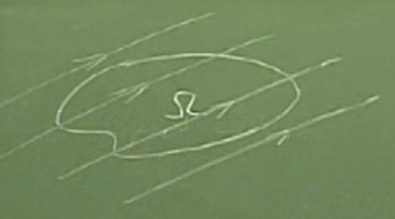
\includegraphics[height=2cm]{1_1.png}

$\mathbb{R}^n$'deki bu sabit hiz alanini $\vec{V}$ olarak gosterelim. $\vec{V}$'nin vektor isaretini 
koyduk, ama ileride bunu yapmayabiliriz, ama anlatimin cercevesinden bir
seyin  vektor olup olmadigini anlamak kolay. 

Yani bu siviyi olusturan parcacikler ayni / esit (uniform) hizda hareket
ediyorlar. 

Sivinin $x$ noktasindaki $t$ anindaki yogunlugu $\rho(x,t)$ olarak
gosterilsin. O zaman $t$ aninda $\Omega$ alanindaki kutleyi hesaplamak
istiyorsam, o zaman yogunlugun hacim uzerinden entegralini alirim. 

\[ \textit{Kutle } = \int_\Omega \rho(x,t) dx \]

Birimleri kontrol edeli, $\rho(x,t)$ kutle / hacim (mesela $kg / cm^3$)
birimine sahip, hacim uzerinden entegral alinca elimize kutle gecer. 

Bu sivi belirlenen alan uzerinden surekli akiyor. O alan icindeki kutlenin
degisim oranini merak ediyorum. Su hesabi yapmam lazim

\[ \frac{d}{dt} \int_\Omega \rho(x,t) dx   \]


Degisim orani $\Omega$ bolgesinin sinirlarindan ne geciyorsa o'dur. 

Bolgenin dis sinirina dik olan birim normal vektorler dusunelim. Eger bu
vektorlerden kirmizi okla gosterilen soldaki normale bakarsak, sivi akisi
ona pek etki etmiyor, yani zarin o bolgesinde cikis fazla yok. Fakat sagda
isaretli normal uzerinden oldukca fazla akis var.

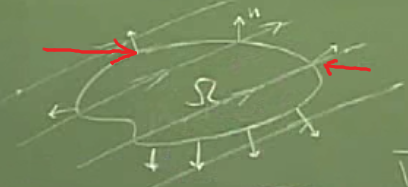
\includegraphics[height=3cm]{1_2.png}

Bu durumu da

\[ \frac{d}{dt} \int_\Omega \rho(x,t) dx   = 
- \int_{\partial \Omega} \rho(x,t) \vec{v} \cdot \vec{n} \ dS 
\]

seklinde gosterebiliriz (esitligin sag tarafini simdi ekledik). $\partial
\Omega$ bolgenin 
``siniri'' anlaminda kullanildi, eger 2 boyutlu duzlemde isek
$\partial \Omega$ siniri bir egridir, eger 3 boyutta isek sinir 2 boyutlu bir
yuzey (surface), vs (genel kural olarak $n-1$ boyutlu bir yuzeydir).

$\vec{n}$ resimde cizilen birim normaller. 

Bu denklemin tek soyledigi iceri giren ile cikanin birbirine (eksi isaret
sonrasinda) birbirine esit oldugu. Iki tarafin kutle / zaman birimine sahip
oldugunu kontrol edebiliriz. 

Simdi Ileri Calculus'tan hatirlayabileceginiz bir kural 

Gauss'un Teorisi

$F: \mathbb{R}^n \to \mathbb{R}^n$ uzerinde tanimli herhangi bir vektor alani icin,
$x
\mapsto F(x)$ olmak uzere, $\mapsto$ isareti eslenme (maps to) anlamina
geliyor, $\Omega \subset \mathbb{R}^n$ bolgesi var ise, ve bu vektor alani
puruzsuz (smooth) bir vektor alani ise (bu vektor bilesenlerinin
turevi alinabilir fonksiyonlar oldugunu soyler), o zaman su da
dogrudur. Vektor alaninin sapmasini (divergence) entegre ediyorum, 

\[ 
\int_\Omega \nabla \cdot F \ dx =
\int_{\partial \Omega} F \cdot n \ dS
\]


$\nabla \cdot$ operatoru $div$ anlaminda kullanildi, ve $\Omega$ bir alan. 

Gauss'un Teorisi, Calculus'un Temel Teorisinin cok boyutlu bir karsiligi
olarak dusunulebilir aslinda.

Gauss'un Teorisini bizim formulasyona uygulayalim

\[ \int_{\partial \Omega} \rho \vec{v} \cdot \vec{n} \ dS =
\int_\Omega \nabla \cdot (\rho \vec{v}) dx 
\]

Simdi sunu yazabilirim

\[ \frac{d}{dt} \int_\Omega \rho \ dx = 
\int_\Omega \nabla \cdot (\rho \vec{v}) dx
 \]

Esitligin solundaki turevi alip, sag tarafi sola tasiyalim

\[ \int_\Omega \bigg( 
\partial_t \rho + \nabla \cdot (\rho \vec{v}) 
\bigg)dx = 0
 \]

$\Omega$ isareti $\mathbb{R}^n$ icinde herhangi bir hacim ise (iki boyutta bir
alan, 3 boyutta hacim), bu hacimi sonsuz kuculttugumuzde artik su ifadenin 

\[ \partial_t \rho + \nabla \cdot (\rho \vec{v})  = 0 \]

noktasal (pointwise) olarak her $x,t$ icin dogru oldugunu gorebiliriz, eger
$\rho$ yeterinc puruzsuz bir fonksiyon ise tabii ki. 

Ustteki fonksiyon suna da esittir

\[ \partial_t \rho + \vec{v} \cdot \nabla \rho = 0\]

Bu denklem $F(x,\rho,\nabla \rho)=0$ formundaki bir denklemdir, genel
olarak bu formla ilgileniriz, bir ustteki ornek ise bu formun en basit
orneklerinden biri, transportasyon fenomeni (transport phenomena) denklemi.

Simdi transport denklemini cozelim, once direk olarak, sonra biraz dolayli
gibi gozukebilecek bir sekilde ama sonra gorecegiz ki bu dolayli yontem
aslinda cozum icin cok uygun. 

Tek boyutta formul su formda

\[ \partial_t \rho + v \partial_x \rho = 0 \]

Daha genel olarak diyelim ki 

\[ \partial_t u + c\partial_x u = 0, \ \ c>0 \]

var diyelim, baslangic sarti

\[ u(x,0) = F(x) \]

Boyle problemlere cogunlukla Baslangic Sart Problemleri (Initial Value
Problem) ismi verilir. 

Diyelim baslangic sarti $F \in C'$  soyle bir fonksiyon

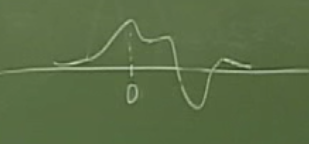
\includegraphics[height=2cm]{1_3.png}

Cozum nedir? Sudur 

\[ u(x,t) = F(x-ct) \]




















\end{document}
